\documentclass[./main.tex]{subfiles}
% \vspace{\baselineskip}
\begin{document}

\chapter{INTRODUCTION}

\section{Overview}
In today’s dynamic financial landscape, capital markets provide individuals with a compelling avenue to actively engage in economic activities, especially through investments. Among the various investment options available, stocks emerge as a prominent choice, representing ownership in companies. The returns realized by stockholders are intricately tied to the financial performance of these entities, creating a straightforward equation: when companies thrive, so do their stockholders. However, the promise of significant profits in the stock market is accompanied by greater investment risk. This underscores the increasing importance of predicting future stock prices based on past data. This proposal aims to leverage the capabilities of machine learning to address this critical issue.\cite{momin2019stock}
\medskip
\newline
\noindent
The price movements of stocks are not isolated events; they are deeply intertwined with the broader economic landscape.
Factors such as monetary policy, influenced by variables like the amount of money in circulation and interest rates, as well as fiscal policy, including taxation policies, play pivotal roles in shaping the behaviour of stock investors.\cite{ticknor2013bayesian}
\medskip
\newline
\noindent
In the not-so-distant past, various methodologies such as linear regression, time-series analysis, and even chaos theory have been applied to predict stock prices. Yet, with the advent of machine learning, we stand at the threshold of a transformative era in stock price prediction. This project explores how cutting-edge machine learning algorithms and techniques can revolutionise our ability to forecast stock prices accurately, empowering investors with invaluable insights and enabling them to make informed decisions in an ever-evolving financial ecosystem.

\section{Problem Statement}
The challenge at hand is to develop an accurate and reliable method for predicting future stock prices in a volatile financial market. 
The allure of potentially high returns in the stock market is counterbalanced by the inherent risks, making it imperative to find a robust solution that leverages historical data and machine learning techniques to make informed predictions. 
\medskip 
\newline
\noindent 
The primary challenge is the development of an accurate and precise stock price prediction model that can effectively capture the complex interplay of market factors, including economic indicators, geopolitical events, corporate earnings, and investor sentiment.\cite{mohammed2020challenges} 
\medskip 
\newline
\noindent
Moreover, it's widely recognized that managing risk plays a crucial role in investing. With the stock market being so unpredictable, investors need tools to understand and reduce risks effectively. This involves thorough testing and refining the model to make it more accurate and reliable. Dealing with real-time predictions means considering factors like data delays, improving the model continuously, and strategies for using the latest information. Also, it's important to provide user-friendly charts and reports to help investors understand and act on the predictions. To follow the rules and regulations, we make sure we're in line with financial laws. In the end, our approach aims to help investors make well-informed decisions and manage risks in the ever-changing world of financial markets.

\section{Objectives}
\begin{enumerate}[label=\textasteriskcentered]

    \item To develop analytical tools for market insights, real-time strategy adjustments, and robust risk assessment.
    \item To Create accurate predictive models using AI and continuous improvement mechanisms for reliable and transparent stock investment forecasts.
    \item Enable dynamic scenario analyses, provide market unpredictability education, and implement adaptive strategies for changing market conditions.
\end{enumerate}

\section{Scope and Limitations}
\subsection{Scope}
\begin{enumerate}[label=\textasteriskcentered]
    \item \textbf{Web Based platform}:Our application will be accessible via the internet, providing a web-based platform.
    \item \textbf{Educational Component}: In addition to prediction, the application may offer educational resources and insights to help users understand the factors affecting stock prices and improve their investment knowledge.
   \item \textbf{ Advanced Prediction Models}: Continuous improvement and integration of advanced prediction models to enhance the accuracy of stock price forecasts.
 
\end{enumerate}
\subsection{Limitations}
\begin{enumerate}[label=\textasteriskcentered]
    \item \textbf{Accuracy}: The accuracy of the proposed system is highly dependent on that of algorithm used and Quality of Data.  
    \item \textbf{Market Volatility}: The stock market is subject to high volatility, and the application may not be able to account for extreme market conditions or sudden economic changes that can significantly affect stock prices.
    \item \textbf{Historical Data Dependency}:The accuracy of predictions heavily relies on historical data. If there are data gaps or inaccuracies in the historical NEPSE data, it may impact the reliability of the predictions.
\end{enumerate}

\section{Motivation}
Stock price prediction is a longstanding and crucial problem. Crafting a dependable model for predicting stock prices can provide valuable insights into how the market behaves over extended periods, helping us identify trends that might otherwise go unnoticed. With the increasing computing power of today's machines, machine learning emerges as an effective approach to address this challenge. Consequently, our inspiration arises from the aspiration to establish a public service that harnesses historical data and user predictions to construct a more resilient model, ultimately benefiting a broader audience.

\section{Development Methodology}
A system development model, also known as a software development life cycle (SDLC) model, is a framework that outlines the processes involved in the planning, creation, testing, deployment, and maintenance of a software system. The purpose of these models is to provide a structured approach to guide the development process, ensuring that software projects are well-organized, efficient, and result in high-quality products.
\subsection{Agile Model}
The Agile model is an iterative and incremental approach to software development. It emphasizes collaboration, flexibility, and customer feedback throughout the development process.
The Agile model is well-suited for our stock prediction application due to the following reasons:
\begin{enumerate}[label=\textasteriskcentered]
\item \textbf{User-Centric Approach}: Agile places a strong emphasis on customer feedback and involvement
  \item   \textbf{Flexibility}: Agile allows for changes and adaptations as the project progresses. This flexibility is valuable for a stock prediction application because financial markets are dynamic and frequently updating.
  \item \textbf{Research and Development}: Agile encourages a culture of continuous improvement. Which encourages our team to regularly reflect on their processes and seek ways to enhance efficiency and  with continious improvement approach.\cite{boehm2007survey}
 
\end{enumerate}
 \begin{figure}[H]
     \centering
     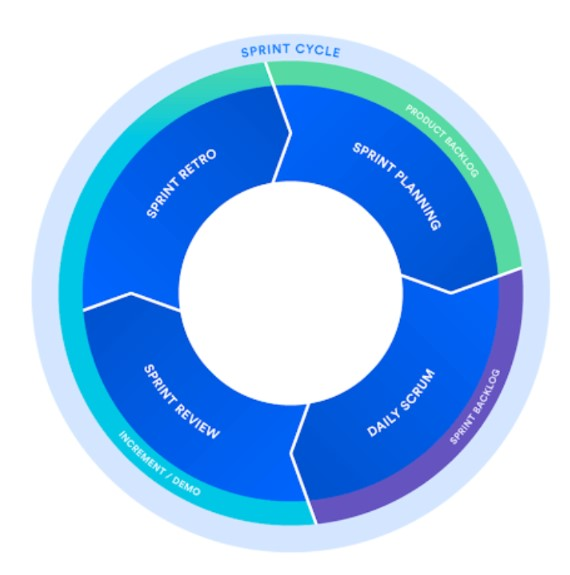
\includegraphics[width=0.75\linewidth]{images/Diagram-or-visual-representation-of-a-Scrum-sprint.jpg}
     \caption{Agile Development}
     \label{fig:3.1}
 \end{figure}
 During our project development, we adopted the Agile methodology, specifically leveraging the Scrum framework. Scrum, named after the rugby formation, is a framework designed to facilitate teamwork. Similar to a rugby team preparing for a match, Scrum encourages teams to learn from experiences, self-organize while tackling problems, and reflect on both successes and setbacks for continuous improvement.
 In line with the Scrum framework, we organized our project into sprints, each being a time-boxed effort with a predefined duration. Typically, the duration ranged from one week to one month, with two weeks being the most common.
 Throughout the development process, we conducted several collaborative sessions and utilized Trello as our chosen project management tool. Trello is a versatile software that helps software teams plan, track, and manage their work by breaking it down into manageable tasks. With Trello, we seamlessly created user stories, managed issues, planned sprints, and efficiently distributed tasks across our software team.
 This approach facilitated a systematic development process for our project, encouraging seamless collaboration with field experts and our project supervisor.
 
 \section{Organization of the Report}
    This report is organized into six chapters.
   \newline \noindent First Chapter introduces the project, outlining the problem statement, objectives, scope, and limitations. It also provides an overview of the development methodology and the motivation behind the project.
   \newline \noindent
   Second Chapter presents a comprehensive review of the literature, exploring the various methodologies and techniques used in stock price prediction.
   \newline \noindent Third Chapter delves into the methodology, detailing the approach and techniques used in the development of the stock price prediction model.
   \newline \noindent Fourth Chapter provides an in-depth analysis of the system architecture, outlining the system's components and their interactions.
    \newline \noindent Fifth Chapter discusses the implementation of the stock price prediction model, detailing the tools and technologies used in the development process.
   \newline \noindent Sixth Chapter concludes the report, summarizing the findings and discussing the implications of the stock price prediction model.
\end{document}